\documentclass[12pt]{article}
\usepackage[utf8]{inputenc} % default from sharelatex
\usepackage{indentfirst} % to indent fist paragraph
\usepackage[brazilian]{babel} % BR
\usepackage{graphicx} % to have pictures

\graphicspath{{images/}}

\title{Sobre o DES}
\author{Lucas João Martins}
\date{}

\begin{document}

\maketitle

\section*{}
\subsection*{1. (3.7) Show that DES decryption is, in fact, the inverse of DES
encryption.}

  A constatação de que o decifrador do DES é o inverso do cifrador do DES pode
  ser alcançada facilmente após a observação dos passos de cada uma das etapas,
  onde fica visível que enquanto um lado possui etapas em uma sequência X, o
  outro lado possui etapas em uma sequência contrária de X. Além disso, sabe-se
  que IP é o inverso de IP\textsuperscript{-1}, fato que ajuda na comprovação
  dessa inversão entre cifrador e decifrador.

\subsection*{2. (3.9) Consider the substitution defined by row 1 of S-box
S\textsubscript{1} in Table S.2. Show a block diagram similar to Figure 3.2 that
corresponds to this substitution}

  \begin{figure}[h]
    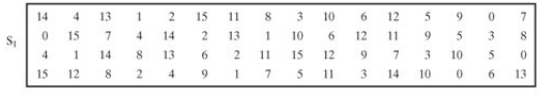
\includegraphics[width=\linewidth]{des_block_substitution}
    \caption{S-box S\textsubscript{1}}
  \end{figure}

  \begin{figure}[h]
    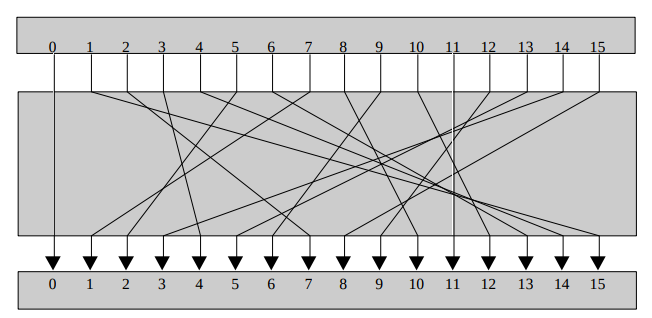
\includegraphics[width=\linewidth]{des_block_diagram}
    \caption{Resposta}
  \end{figure}

\subsection*{3. (3.10) Compute the bits number 1, 16, 33, and 48 at the output
of the first round of the DES decryption, assuming that the ciphertext block is
composed of all ones and the external key is composed of all ones.}

  \begin{itemize}
    \item Chave K = 11...11 (56 bits)
    \item Chave após cada round K\textsubscript{1} = ... = K\textsubscript{16} =
    11...11 (48 bits)
    \item Texto cifrado C = 11...11 (64 bits)
    \item Entrada no primeiro round para decifrar = 11...11 (64 bits)
    \begin{itemize}
      \item LD\textsubscript{0} = RD\textsubscript{0} = 11...11 (32 bits)
    \end{itemize}
    \item Saída do primeiro round (conforme livro) =
    LD\textsubscript{1}RD\textsubscript{1}
    \begin{itemize}
      \item LD\textsubscript{1} = RD\textsubscript{0} = 11...11 (32 bits)
      \item RD\textsubscript{1} = LD\textsubscript{0} + F(RD\textsubscript{0},
      K\textsubscript{16})
    \end{itemize}
    \item \textbf{Os bits 1 e 16 são provenientes de LD\textsubscript{1}, logo
    são iguais a `1'}
    \item Por outro lado, os bits 33 e 48 são os bits 1 e 16 de
    RD\textsubscript{1}
    \begin{itemize}
      \item Após análise pode-se perceber que o bit 1 da função F vem da quarta
      saída de S4, enquanto que o bit 16 dessa mesma função vem da segunda saída
      de S3. Além disso, esses bits fazem XOR com as possições correspondentes
      de LD\textsubscript{0}
      \item A entrada para todas as caixas S é igual a 000000
      \item A saída de S3 é 1010, sendo o bit que buscamos o `0' da segunda
      posição
      \item A saída de S4 é 0111, sendo o bit que buscamos o `1' da quarta
      posição
      \item Após o XOR, o bit que era o 1 da função F é igual a `0', enquanto
      que o bit que era o 16 da função F é igual a `1'
    \end{itemize}
    \item \textbf{No fim, o bit 33 é igual a `0' e o bit 45 é igual a `1'}
  \end{itemize}

\subsection*{4. (3.12) Compare the initial permutation table (Table S.1a) with
the permuted choice one table (Table S.3b). Are the structures similar? If so,
describe the similarities. What conclusions can you draw from this analysis?}

  \begin{figure}[h]
    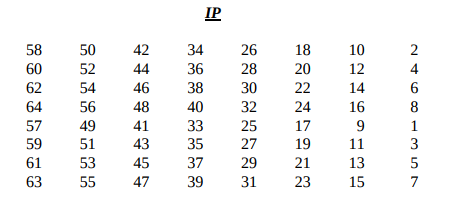
\includegraphics[width=\linewidth]{des_ip}
    \caption{Initial permutation table (Table S.1a)}
  \end{figure}

  \begin{figure}[h]
    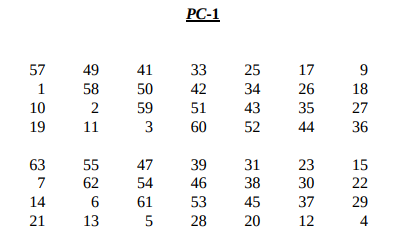
\includegraphics[width=\linewidth]{des_pc_1}
    \caption{Permuted choice one table (Table S.3b)}
  \end{figure}

  As estruturas são muito similares, na verdade são praticamente iguais, mas
  possuem algumas diferenças:
  \begin{itemize}
    \item PC\textsuperscript{-1} não possui uma oitava coluna
    \item os números são iguais, mas as suas posições diferem entre as duas
    tabelas
  \end{itemize}
  A principal conclusão após verificar essa similaridade é de que esse fato pode
  permitir uma implementação parecida entre as duas.

\subsection*{5. (3.15) Show that in DES the first 24 bits of each subkey come
from the same subset of 28 bits of the initial key and that the second 24 bits
of each subkey come from a disjoint subset of 28 bits of the initial key.}

  Basta observar a tabela de escolha de chave no DES (\textit{compreension
  D-box}), onde é visto que os primeiros 24 bits são selecionados dos primeiros
  28 bits e os últimos 24 bits são selecionados dos últimos 28 bits.

  \begin{figure}[h]
    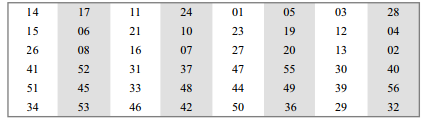
\includegraphics[width=\linewidth]{des_key_table}
    \caption{Tabela de escolha de chave no DES}
  \end{figure}

\subsection*{6. (3.16) Refer to Figure G.2, which depicts key generation for
S-DES.}

  \subsubsection*{a. How important is the initial P10 permutation function?}

    Perceba que antes da realização de P10 existem 2\textsuperscript{10}
    possíveis chaves únicas. Após a aplicação de P10, que se trata de uma
    permutação simples, ainda irá existir 2\textsuperscript{10} possíveis chaves
    únicas. Com isso, essa permutação não adiciona em nada na segurança do
    algoritmo.

  \subsubsection*{b. How important are the two LS-1 shift functions?}

    Pelo mesmo motivo explicado na resposta da alternativa anterior, os dois
    deslocamento a esquerda de 1 bit não adicionam em nada na segurança do
    algoritmo.

\subsection*{7. (3.18) Using S-DES, decrypt the string (10100010) using the key
(0111111101) by hand. Show intermediate results after each function (IP,
F\textsubscript{K}, SW, F\textsubscript{K} , IP\textsuperscript{-1}). Then
decode the first 4 bits of the plaintext string to a letter and the second 4
bits to another letter where we encode A through P in base 2 (i.e., A = 0000, B
= 0001, ..., P = 1111). Hint: As a midway check, after the application of SW,
the string should be (00010011).}

  Geração das subchaves:
  \begin{itemize}
    \item chave = 0111111101
    \item P10 = 1111110011
    \item Shift = 1111100111
    \item P8 = 01011111
    \item \textbf{K\textsubscript{1} = 01011111}
    \item Shift = 1111111100
    \item P8 = 11111100
    \item \textbf{K\textsubscript{2} = 11111100}
  \end{itemize}

  Processo de decifrar:
  \begin{itemize}
    \item Texto cifrado = 10100010
    \item IP = 00110001
    \item F\textsubscript{K}:
    \begin{itemize}
      \item E/P = 10000010
      \item E/P xor K\textsubscript{2} = 01111110
      \item S0 = 00
      \item S1 = 00
      \item P4 = 0000
      \item P4 xor 4 bits iniciais da entrada = 0011
      \item Saída = 00110001
    \end{itemize}
    \item SW = 00010011
    \item F\textsubscript{K}:
    \begin{itemize}
      \item E/P = 10010110
      \item E/P xor K\textsubscript{1} = 11001001
      \item S0 = 01
      \item S1 = 10
      \item P4 = 0110
      \item P4 xor 4 bits iniciais da entrada = 0111
      \item Saída = 01110011
    \end{itemize}
    \item IP\textsuperscript{-1} = 10101110
    \item Texto original = 10101110
    \item Texto traduzido = JN
  \end{itemize}
\end{document}
